\documentclass[10pt,twocolumn,letterpaper]{article}

\usepackage{cvpr}
\usepackage{times}
\usepackage{epsfig}
\usepackage{graphicx}
\usepackage{amsmath}
\usepackage{amssymb}

% Include other packages here, before hyperref.

% If you comment hyperref and then uncomment it, you should delete
% egpaper.aux before re-running latex.  (Or just hit 'q' on the first latex
% run, let it finish, and you should be clear).
\usepackage[breaklinks=true,bookmarks=false,colorlinks=true]{hyperref}

\cvprfinalcopy % *** Uncomment this line for the final submission

\def\cvprPaperID{****} % *** Enter the CVPR Paper ID here
\def\httilde{\mbox{\tt\raisebox{-.5ex}{\symbol{126}}}}

% Pages are numbered in submission mode, and unnumbered in camera-ready
%\ifcvprfinal\pagestyle{empty}\fi
\setcounter{page}{4321}
\begin{document}

%%%%%%%%% TITLE
\title{CNN-based analysis of organoid growth}

\author{Shan Zhou \\
Facebook \\
\\
{\tt\small shanzhou@stanford.edu}
% For a paper whose authors are all at the same institution,
% omit the following lines up until the closing ``}''.
% Additional authors and addresses can be added with ``\and'',
% just like the second author.
% To save space, use either the email address or home page, not both
\and
Timothy Daley \\
Stanford University \\
Departments of Statistics and Bioengineering \\
{\tt\small tdaley@stanford.edu}
\and
Alexandra Sockell \\
Stanford University \\
Department of Genetics \\
{\tt\small asockell@stanford.edu}
}


\maketitle
%\thispagestyle{empty}

%%%%%%%%% ABSTRACT
\begin{abstract}
   High-throughput analysis of imaging data is critical for analysing large data typical of modern biological investigations.  Here we investigate a convolutional neural network-based approach to analyse the growth of organoids based off of imaging data.  
\end{abstract}

%%%%%%%%% BODY TEXT
\section{Introduction}

Predicting tumor growth rate is a first step in determining treatment options for cancer patients.  Fast growing tumors necessarily require more aggressive treatment.  It would be beneficial if patients could avoid aggressive treatments when possible.  

Alexandra Sockell of the Fordyce and Curtis labs in the Bioengineering and Genetics departments, respectively, of Stanford University has developed a microfluidic device to isolate single cells of a tumor and allow them to grow into organoids  within the microwell.  Organoids are three dimensional stem cell-like cultures that organize into a "mini-organ"~\cite{rios2018imaging}, and can be used to study cancer in a more natural environment than traditional cell lines~\cite{drost2018organoids}.
The objective of her research is to study the mechanisms of tumor growth by subjecting a large number of  individual cells to a wide range of treatments and conditions and track their condition by imaging.  She has taken 14 days of imaging over 8 conditions.    For each day, there are approximate 38,000 well images across all conditions.  The number of cells per well is approximately Poisson, with most of the wells not containing any cells, 25\% have one cell, and smaller portion have more than 1.  We believe that the large number of images should provide a sufficient amount of data and information content to apply deep convolution neural network approach.  Our hypothesis is that the state of the cells in the early days should be related to their final state.  Therefore our objective to determine whether the early stages of the organoid can predict the growth rate and final state of the organoid.    

\begin{figure}[b!]
\begin{center}
 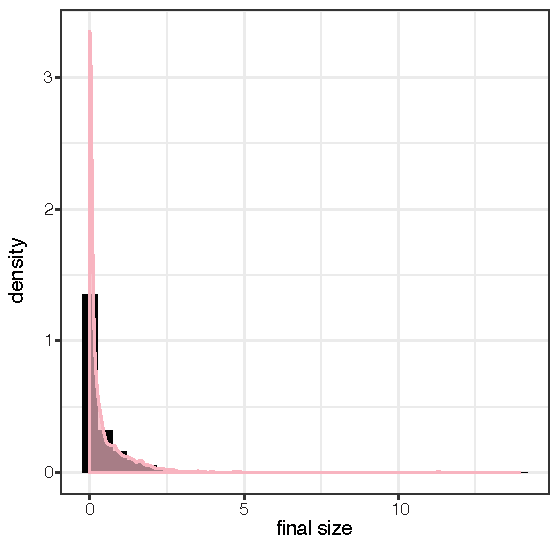
\includegraphics[width=0.8\linewidth]{figures/final_day_hyst2_area_density.pdf}
\end{center}
   \caption{Distribution of normalized final sizes.  There is a large peak at zero corresponding to empty wells or cells that died.}
\label{final_size_dist}
\end{figure}

 \begin{figure*}[t!]
\begin{center}
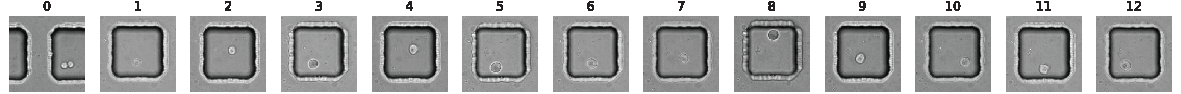
\includegraphics[width=0.9\linewidth]{figures/classification/well_4166_condition_A1_all_days_images_small.pdf}
\end{center}
   \caption{All 14 images from a single microwell.}
\label{well_4166_condition_A1_all_days_images_small}
\end{figure*}

Previous approaches for high-throughput analysis of organoid imaging data did not look at single-cell microwell level data.  Instead they typically relied upon a large number of cells to quantify cell proliferation or death \cite{jabs2017screening},  used cell counting assays to calculate growth \cite{sebrell2018live}, or used single cell tracking to calculate cell motility \cite{geum2016epidermal}.  To our knowledge, no deep learning approaches have been proposed to analyse organoid imaging data, despite the large success in deep learning to analysing imaging data across a broad spectrum of applications.  However, we have found successful convolutional neural network (CNN) approaches in related biological analysis such as high content screening \cite{simm2018repurposing}, but this is not similar enough for us to compare against.



The purpose of this project is to provide a proof of principle for CNN-based high-throughput analysis of organoid imaging data.  



\section{Data}








The data is composed of 193$\times$193 greyscale images of 4800, 3600, 3600, 2400, 3200, 3600 microwells for 6 wells with different experimental conditions, imaged across 14 days (example shown in figure~\ref{well_4166_condition_A1_all_days_images_small}).  So we have 296,800 wells with 14 images per well.  The images were obtained via computational stitching~\cite{preibisch2009globally} of multiple larger images of well.  A small number of images appear distorted.  We filtered the images by the estimated area of their interior, computed by the hyst2 function in openCV~\cite{opencv_library}, to try to reduce such artifacts.  If the estimated area was larger than possible for any of the 14 days, then we removed all images of that well from the data.  After filtering we kept 14,534 microwells.  Example images are shown in figure~\ref{workflow}.

We split the filtered dataset into train validation test set by 8:1:1 with 11,627 training set , 1453 validation set and 1454 test set. For normalization, we get the mean and standard deviation for each day well images across all training set. Then we apply these mean and standard deviation to normalize all training set, validation set and test set. Besides, we also normalize the lable, the final day well cell size for the regression model.

For features, we tried with different single day image and also tried stacking two days or three days well images. For classification label, we determine whether final day has cell by computing whether the hyst2 area is greater than zero. For prediction label, we just use the hyst2 area of final day well. 

One difficulty with this project is that we did not obtain all the data at the start.  We began with one experiment (4800 microwells), and then obtained data from more experiments as they were processed.   We found that some models built on the first experiment did not generalize well, and a major objective is to ensure that our model is generalizable across biological conditions.

 \begin{figure}[b!]
\begin{center}
 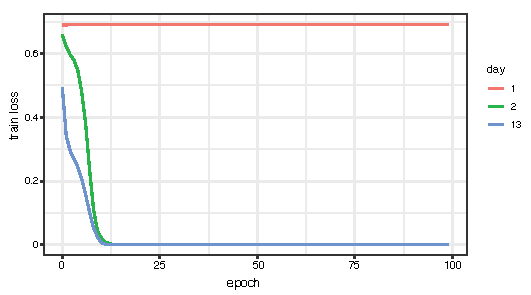
\includegraphics[width=0.9\linewidth]{figures/day13_train_loss_vs_epoch_vs_day_v2.pdf}
\end{center}
   \caption{Cross-entropy loss for the training set using days 1, 2, and 13 to predict whether hyst2 area is zero at day 13.}
\label{train_loss_day_1_2_13}
\end{figure}

%We tried single day image, but day 1 iamge does not work weel. We also tried stacking 2 days or 3 days images for input, the results looks better.

%We normalize the input images and size labels by using the training data mean and standard deviation.

%We added data augmentation by random cropping with different size and horizonal flipping.

 \section{Methods}
 
 \subsection{Proof of principle model}
 \label{proof_of_principle}
 
 To start we approached the regression problem straightforward.  We found difficulties with overfitting using only day 1 on the images from a single well.  We therefore decided to first focus on the classification problem, to predict from the early days whether the final day is empty or not, using whether the computed hyst2 area is zero or not as zero and one, respectively.   As a proof of principle, we attempted to overtrain a deep convolutional neural network consisting of three convolutional layers, with kernel sizes of 2, 3, and 3, respectively, and channels of 64, 32, 16, respectively.  Each convolutional layers was followed by a batch normalization layer, a ReLU layer, and then a max pooling layer with a kernel size of 2.  The convolutional layer were followed by a square fully connected layer, followed by a ReLU layer, a fully connected layer with output size of one, and finally a sigmoid for output.  We applied this network to all images from a single well, and attempted overfitting on day 1, day 2, and day 13, using cross-entropy loss.  Day 13 was included as a sanity check, since the hyst2 area was computed using the day 13 images.  The training loss for days 2 and 13 quickly went to zero, while the loss for day 1 did not go below the loss for random guessing (Figure~\ref{train_loss_day_1_2_13}).  We therefore excluded days 1 and 0 from further consideration because they do not appear to be informative towards our objective.  It may be that day is informative when combined with other days, but not by itself.
 
 \begin{figure*}[t!]
\begin{center}
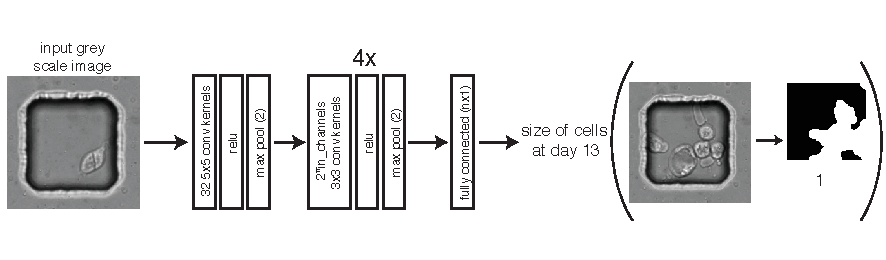
\includegraphics[width=0.8\linewidth]{figures/networkExampleImage_v2.pdf}
\end{center}
   \caption{Example workflow of our CNN algorithm.  The input is a 193$\times$193 greyscale image of the cell at day one.  We pass this through a convolutional neural network to whether the final well is empty, using the hyst2 area as a proxy.}
\label{workflow}
\end{figure*}

\subsection{Deep CNN for multi-day input}
\label{multidayCNN}

After the initial proof of principle we built a classification CNN to predict whether the microwell was empty at the end of the time point (indicating cell death), using hyst2 area as a proxy for whether a cell is empty or not.  If the hyst2 area at day 13 is zero then we say that microwell is empty and if the hyst2 area is greater than zero then we say the microwell is non-empty.  This CNN had five convolutional layers, all with batch normalization, ReLU, and max pooling following, with channels sizes of 32, 64, 128, 256, and 256 and kernel sizes of 5, 3, 3, 3, 3 (Figure~\ref{workflow}).  We used cross-entropy as the loss function and the Adam optimizer with learning rate $10^-4$.   To facilitate generalization of our model we used Dropout regularization with $p = 0.5$.  To take into account the temporal nature of our data we used multiple day images as input.  We treated each separate image as an input channel (since each image is a single grey-scale channel).  We initially used days 2 and day 8 images as input, and later used days 2, 5, and 8 as input.


\subsection{Pretrained model}

We also applied pre-trained models, using transfer learning to train only the final output layer, keeping the other layers constant.  We found success with the ResNet 18 model, but not as good as our previously discussed model.

\subsection{Data augmentation}

Because of the paucity of experiments, we explored data augmentation approaches.  Because the primary information is in the center of the image, we hypothesized that random cropping may be a suitable data augmentation strategy.  Additionally, the information content of the images should be rotation invariant.   Therefore we also explored rotations for data augmentation.


 %After initial models, we generate two models. The first model is a classification CNN model to find out whether the final day wells has cell or not. We built a five convolutional layer with max pooling and one fully connected layer model with dropout. We compute cross-entropy for loss and use Adam for the optimizer. The model is overfitting for 4000 training images. But when the training set increase to 6000, the validation accuracy incresed to around 0.8. However adding more images to 10000 does not makes the model overffiting again. We then tried adding more regulization like more max pooling and dropout. We also added data augmentation to random crop and rotate the images. We add learning rate decay in the optimizer every 5 steps by 0.1. We also use pretrained ResNet18 mode, the validation accuracy did not increase.

% After finding out which wells has cells by classification model, we predict their final cell sizes by CNN regression model. We used the pretrain ResNet18 model,Adam optimizer and mean square error as loss. 
 \section{Experiments}
 
 \subsection{Classification}
 
For classification, first we used one simple 3-conv,1-fully connected layer without any regularization to train 100 images.  We obtained overfitting, as the training loss went to 0 and the training accuracy  went to 1. However, the validation accuracy remained constant, equal to random guessing.  We then added more convolutional layers and more parameters in each of the convolution network, obtaining the model described in section~\ref{multidayCNN},  and training with more data, 4510 microwells.  We obtained 0.19 as the best validation loss , 0.8 as the best training accuracy and 0.6 as the best validation accuracy across all epochs (figure~\ref{classification_train_loss_train_and_val_loss}).  If we run for more epochs, then the training loss goes to zero and the training accuracy goes to one.  However, the validation accuracy does not improve.  This supports the decision of early stopping.  To improve generalization we then added dropout.  This improved the validation accuracy slightly, to 0.65.
However, the best improvement is when we added more microwells to the training.  Then the validation accuracy improved to 0.8.  The test accuracy for this model is 0.77 (figure~\ref{test_set_confusion_matrix}). But it is still a little bit overfitting.
We explored adding data augmentation for this model, but this did not appreciably improve the validation accuracy but lower the training accuracy. We think the reason is that the well images data already has enough noise since some well images are already flipped and some well images lose part of information. We also explored adding more pooling and regularization, but the validation accuracy does not improve.
To avoid overfitting, we can add more different datasets in the future.

To obtain better accuracy, we have tried different optimzer like SGD and Adam. Adam works better. We also tried different learning rate and adding learning rate decay per 5 epoch. But learning rate 1e-4 without any decay returns higher accuracy than others. 
  

 \begin{figure}[b!]
\begin{center}
 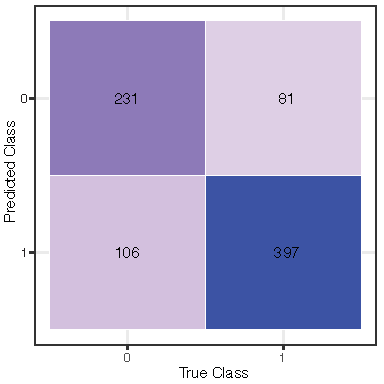
\includegraphics[width=0.9\linewidth]{figures/classification/test_set_confusion_matrix.pdf}
\end{center}
   \caption{Confusion matrix for the classification problem on the 815 microwell test set.}
\label{test_set_confusion_matrix}
\end{figure}



%Then I run for more epoches, the loss almost go to 0 and training accuracy go up to 1 but validation accuracy improves a little bit to 0.65. It was overffiting. So I added dropout and more maxpooling, the validation accuracy went up to 0.68. But it was still overfitting, so I added the training set to 6514. The minum loss is 0.11 and best validation is 0.8 and training accuracy is 0.915. But by changed different models, adding fully connected layer or using pretrained, but validation accuracy did not improve. By adding data augmentation, the training accuracy go down, but validation accuracy did not go up. 
%We have also tried learning rate 1e-2,1e-3,3e-4,1e-4, the best is 1e-4.

 \begin{figure*}[t!]
\begin{center}
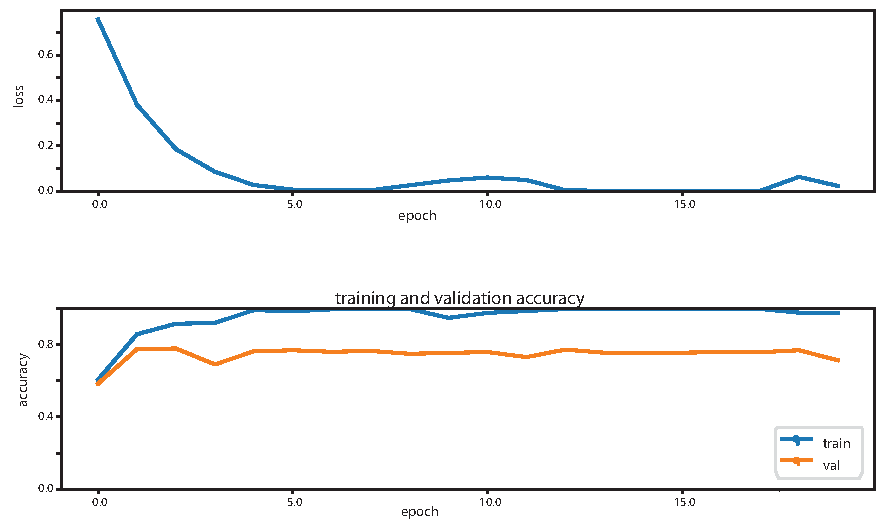
\includegraphics[width=0.8\linewidth]{figures/classification/classification_train_loss_train_and_val_loss.pdf}
\end{center}
   \caption{The training cross-entropy loss (top) and training and validation accuracy (bottom) for the classification problem.}
\label{classification_train_loss_train_and_val_loss}
\end{figure*}

To validate our approach we generated saliency maps for several example images, shown in figure~\ref{saliency_maps}.  We should note that we did not perform data augmentation on any of the images, so that the shifting and rotation shown in the first and last example images are present in the real data.     The saliency maps show a clear indication that the convolutional filters are picking up the signal contained in the microwell.  The boundaries of the microwell contain only noise, and even when the images are rotated or shifted, the interior of the microwell is highlighted in the saliency map.  This is evidence that our convolutional model is correctly identifying the salient information contained in the images.

 \begin{figure}[b!]
\begin{center}
 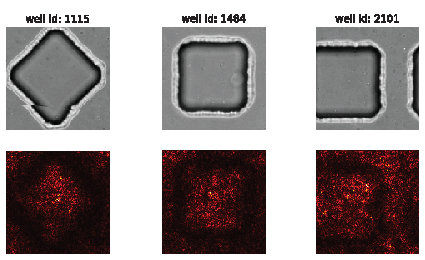
\includegraphics[width=0.9\linewidth]{figures/saliency_maps.pdf}
\end{center}
   \caption{Example images and their corresponding saliency maps.}
\label{saliency_maps}
\end{figure}


\subsection{Regression}

Now that we were satisfied with the results of the classification problem, we turned back to the regression problem.  We took the pretrained ResNet18 for feature generation and used the Adam Optimizer to train the final layer, with mean square error as the loss function.  We looked at only the images that have a final hyst2 area greater than zero.  As discussed in section~\ref{proof_of_principle}, the overabundance of zeros prevented us from directly solving this problem.  We obtained approximately seven thousand microwells for a training set.  We were able to obtain a validation (913 microwells) mean square error of 0.23 after 4 epochs with early stopping (figure~\ref{regression_correlation}).


 \begin{figure}[b!]
\begin{center}
 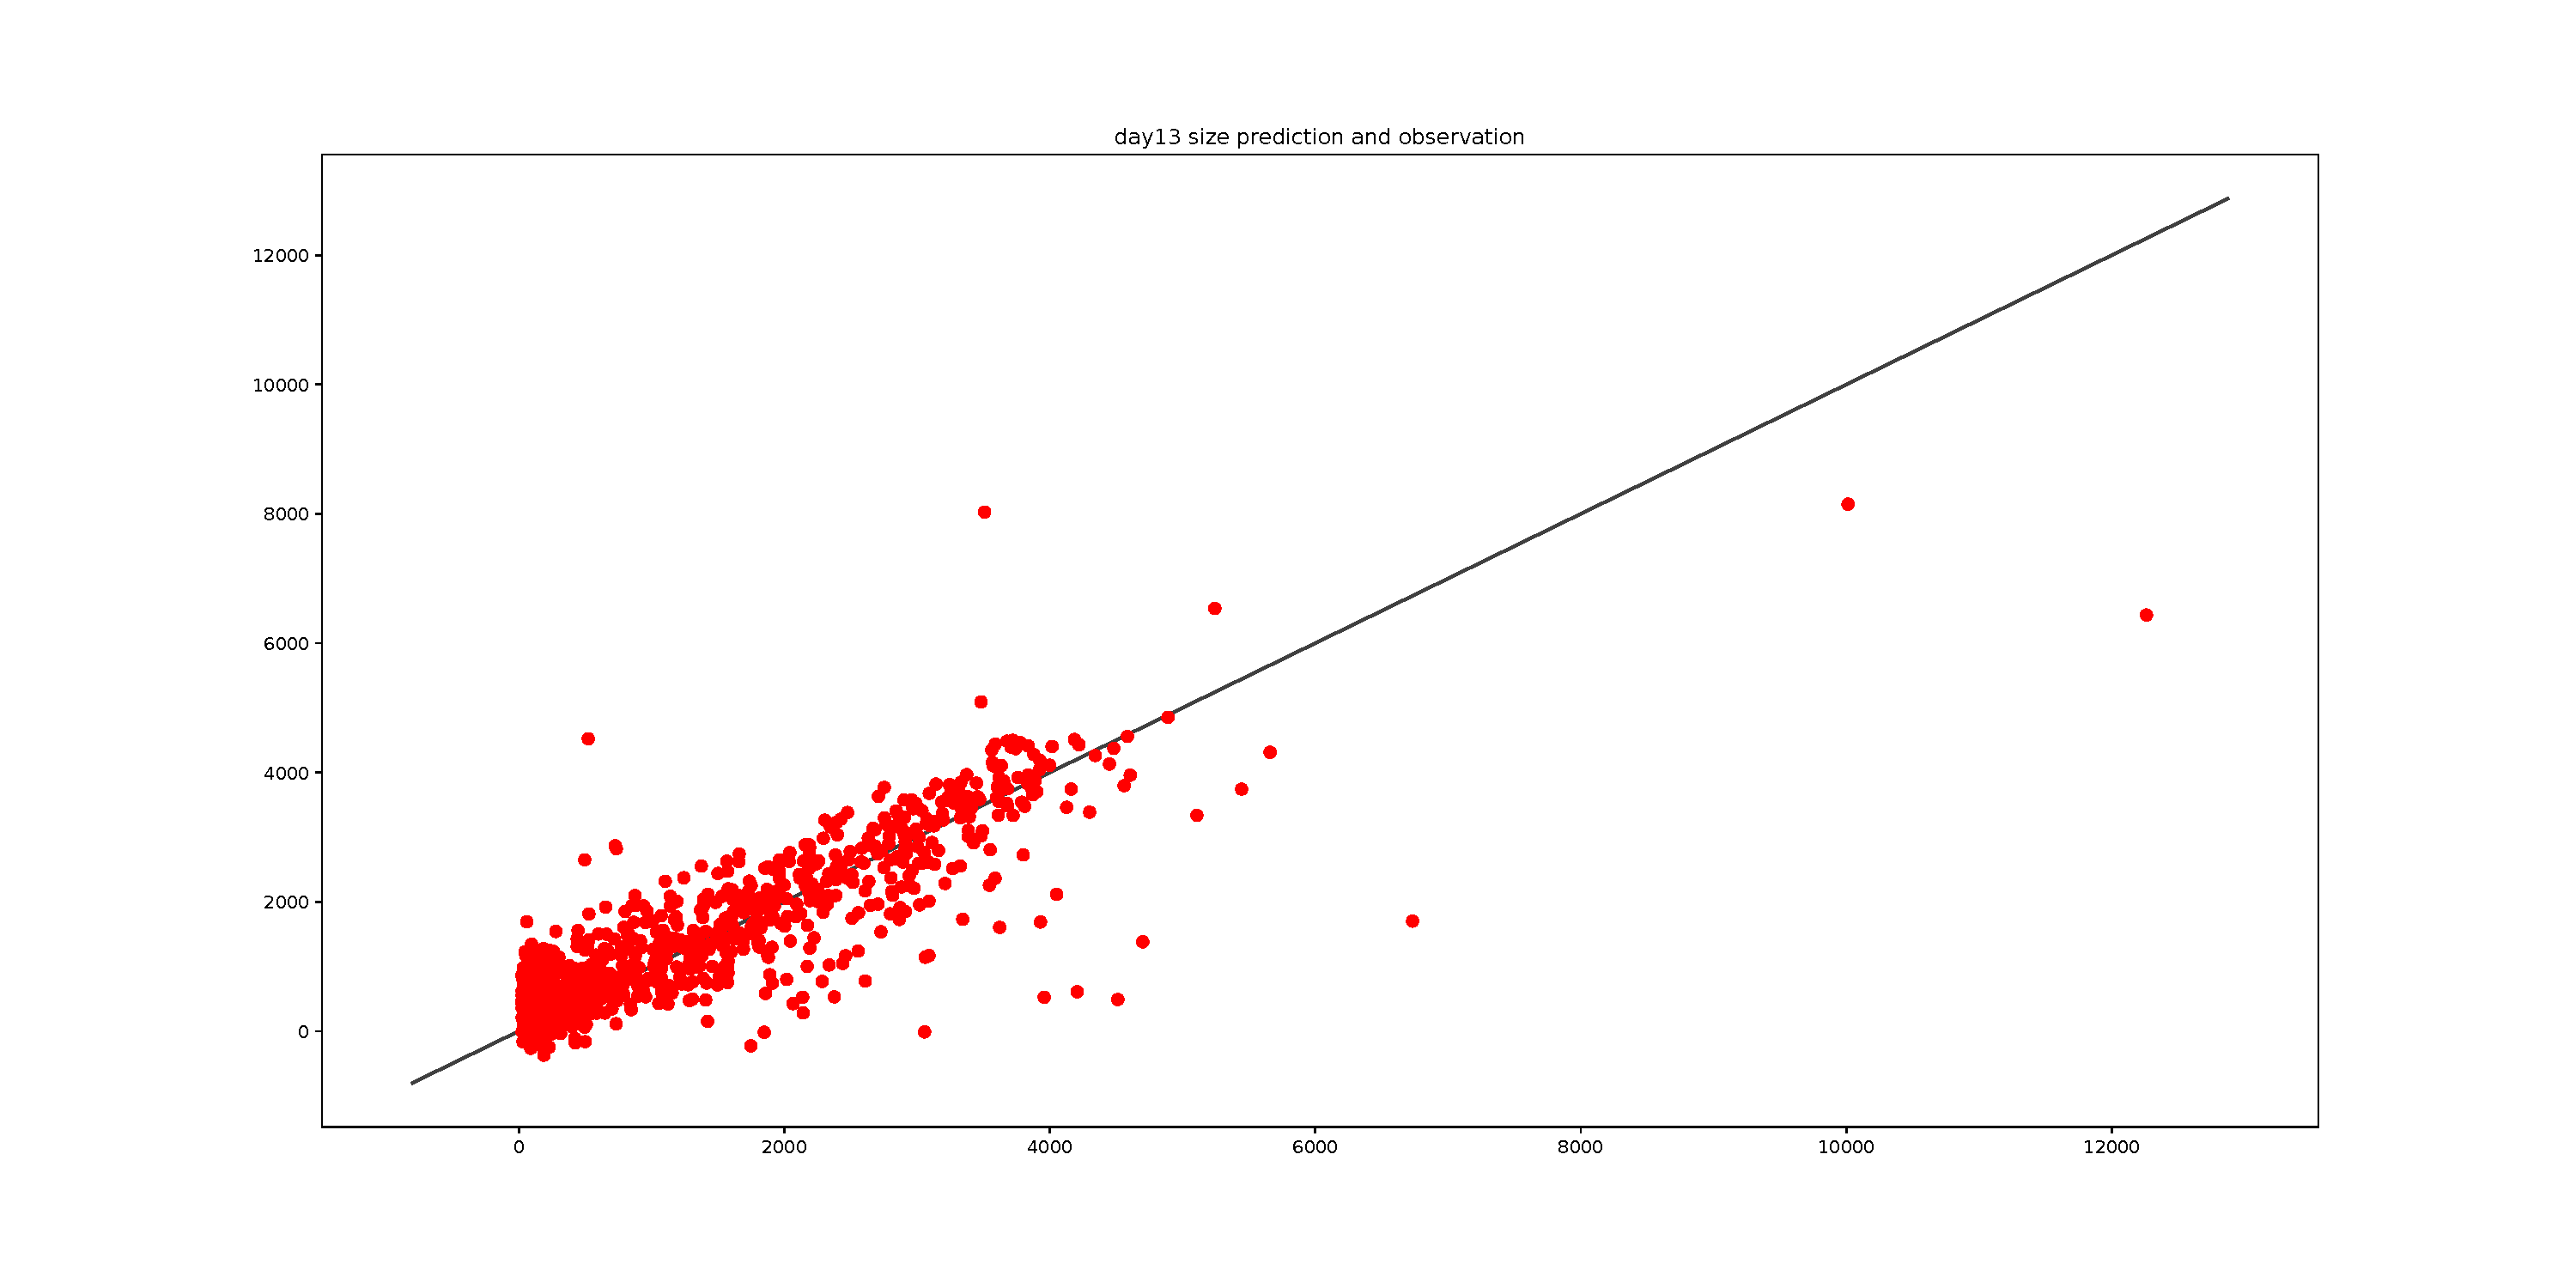
\includegraphics[width=0.9\linewidth]{figures/regression/size_prediction_and_observation_scatter_plot.pdf}
\end{center}
   \caption{The observed hyst2 area size (x-axis) and the predicted hyst2 area size (y-axis) on the validation set.  The correlation is equal to 0.85.}
\label{regression_correlation}
\end{figure}





\section{Conclusions}



This work represents a proof of principle for a CNN approach to microwell image analysis.  We found that the regression problem was difficult to solve in a straight-forward manner due to overabundance of zeros.  We found that using the combination of images from several days improves the predictions.  We found that the pre-trained ResNet18 performed the best, though the performance from our best bespoke model was close behind.  The performance of our models may be inhibited by the fact that we are using a proxy measure for the true size of the cells in the microwell.  Better labeled data will help to improve the performance, as we may be accurately predicting the underlying truth, and just not know it.  


This analysis is complicated by the fact that cells are small in the initial days of the experiment, and this is exactly when the results are most critical for guidance on medical treatment.  We suggest several approaches to improve our results:
\begin{itemize}
\item more data across more biological conditions will help to improve the generalization of the model;
\item better labeling of the true size will help to improve the performance, as there is some inherent variability to the estimated label;
\item because the label we used is inherently noisy, using a GAN to predict the final day image may be a better approach (though this would have been a futile effort with the amount of data that we had);
\item combining the classification and regression problem, possibly by using something similar to a zero-inflated model likelihood as the loss function.
\end{itemize}







{\small
\bibliographystyle{ieee}
\bibliography{bib}
}

\section{Contributions}

A.S. developed the microwell and imaging system and obtained the imaging data.  S.Z. and T.D. developed the methods, performed the analysis, and wrote the paper with input from A.S.  

\end{document}
